\section{Event Cameras}
\label{sec:sec2_event}

Event cameras, also called neuromorphic cameras, silicon retina or dynamic vision sensor (DVS) are image sensors that respond to changes in brightness in the scene. Unlike conventional cameras, which capture full image frames at a fixed frequency (commonly 30Hz or 60Hz), producing redundant information and require a high bandwidth for transmission, each pixel in an event-based camera operate independently and asynchronously, reacting to changes of brightness in the scene, eliminating the transmission of redundant information, allowing for much higher temporal resolution (in the order of microseconds, as opposed to the milliseconds of conventional cameras).

Event cameras are inspired by the behaviour of the cells in the retina. Though oversimplified, retinal cells respond to changes in the environment (namely brightness), generating an electrical impulse. The transient response of each retinal cell is independent. Event cameras mimic this behaviour by asynchronously and independently responding to changes in brightness in the environment, generating ON/OFF events each time a predefined threshold in brightness is exceeded.

This architecture allows for interesting properties, such as microsecond temporal resolution, high dynamic range (above 120dB), which allows for scenes with both bright and dark zones, and does not suffer from under/overexposure, nor motion blur.

Events are triggered when the brightness in a certain pixel surpasses a certain threshold. In particular, discrete brightness steps are pre-defined, and whenever brightness detected crosses the threshold, an event is generated. Positive crossings generate ON events, and negative crossings generate OFF events. In effect, each pixel is constantly working as a comparator (with corresponding electronic to support this mode of working). Fig.\,\ref{fig:sec2_event_camera} shows the first-generation DVS sensor, with an array of 128x128 pixels (from \cite{lichtsteiner2008128}), where this idea of comparison and threshold is shown.

\begin{figure}[ht]
    \centering
    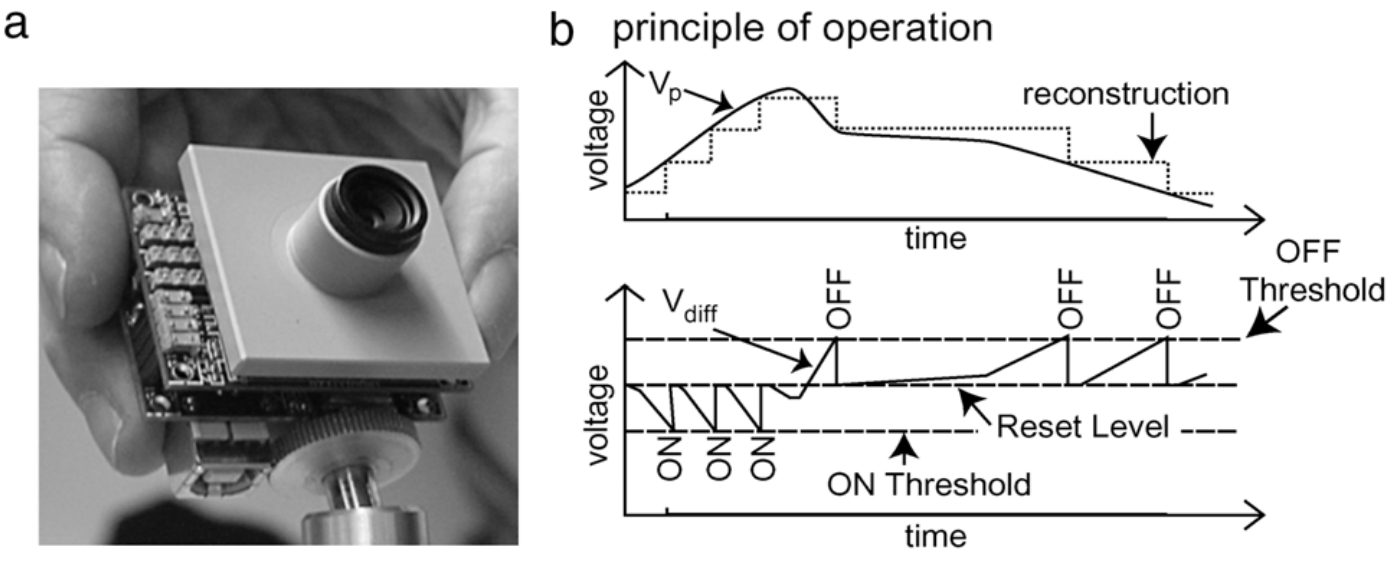
\includegraphics[width = 1\linewidth]{event_camera_principle.PNG}
    \caption[Event camera and operation principle]{First generation event camera (a) and corresponding principle of operation, showing the thresholds and the corresponding asynchronous generation of ON/OFF events, from \cite{clady2015asynchronous}}
    \label{fig:sec2_event_camera}
\end{figure}

Events are then defined as a four-component vector:

\begin{equation}
    \textbf{e} = \left(\left(x,y\right)^T,t,pol\right)^T = \left(\textbf{p},t,pol\right)^T
\end{equation}

The component $p=\left(x,y\right)^T$ refers to the spatial position of the event in the camera. The component $t$ refers to the timestamp of the event, and is of extreme importance due to the microsecond temporal resolution of the camera. Lastly, the parameter $pol$ refers to the polarity of the event (ON/OFF events).

With this event structure, it is common to represent events in a three-dimensional (space-time), representation, as shown in Fig.\,\ref{fig:sec2_space_time}, which shows the space-time evolution of events generated from a rotating black bar on a white background.

\begin{figure}[ht]
    \centering
    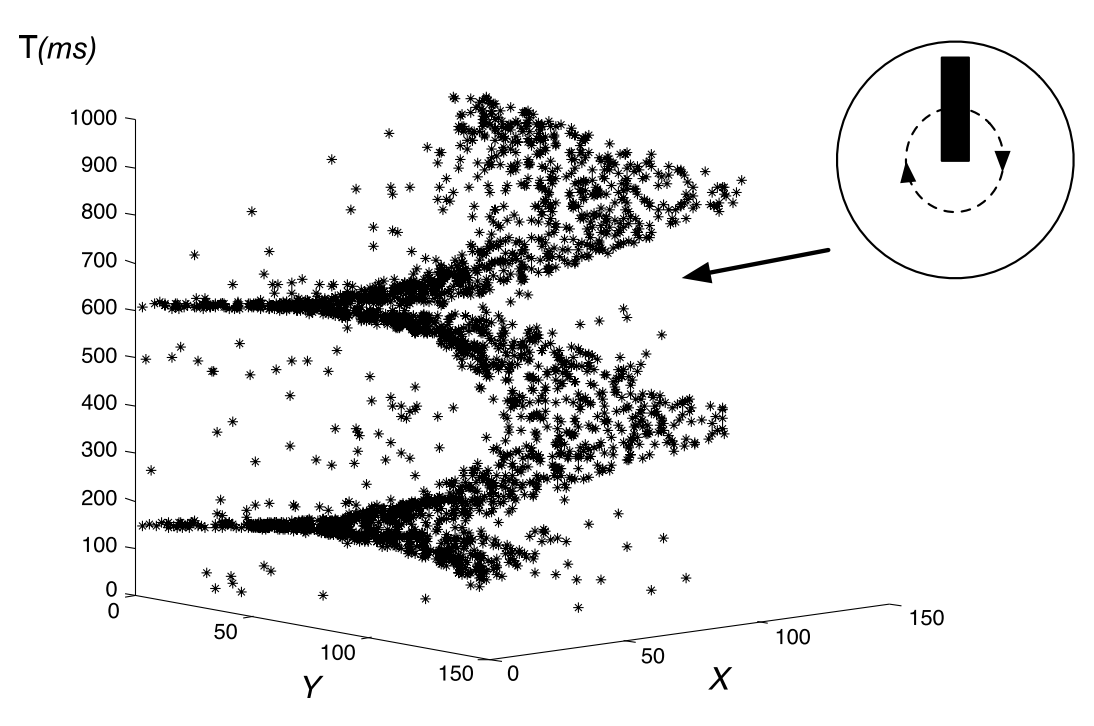
\includegraphics[width = 1\linewidth]{bar_rotating.PNG}
    \caption[Space-time representation of events generated from a rotating black bar]{Space-time representation of events generated from a rotating black bar, from \cite{clady2015asynchronous}}
    \label{fig:sec2_space_time}
\end{figure}

Conventional cameras and event cameras have fundamentally different modes of operation and output. As such, a comparison of the behaviour in the same scene, and an analysis of the output, is interesting. Fig.\,\ref{fig:sec2_standard_vs_event} shows the response of both a conventional camera and an event camera when presented with a disk rotating at a high speed, with a black dot. The fixed capture of the conventional camera is unable to keep up with the speed of the dot, and the images suffer from motion blur (not represented) and some discontinuity between frames. The event camera, however, due to its asynchronous event generation and temporal resolution, is able to continuously produce events relating to the movement of the dot.

\begin{figure}[ht]
    \centering
    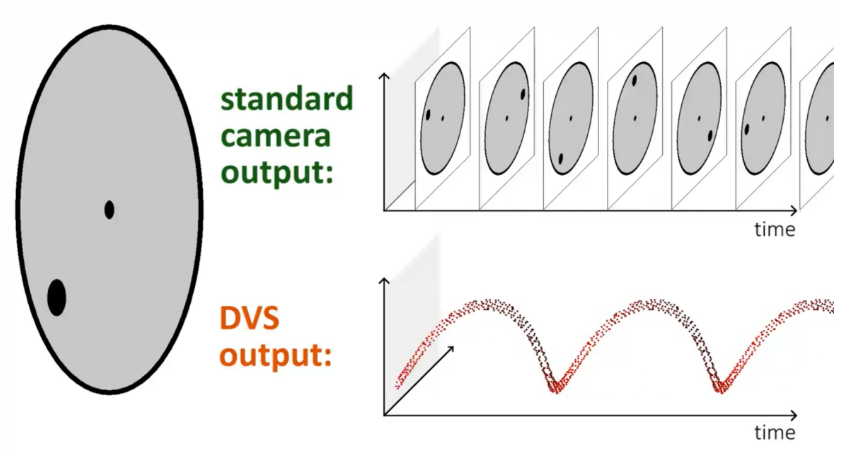
\includegraphics[width = 1\linewidth]{standard_vs_event.PNG}
    \caption[Comparison of the output of a standard camera and an event camera]{Comparison of the output of a standard camera (above), and an event camera (below), when recording a rotating disk with a black dot, from \cite{mueggler2017fast}}
    \label{fig:sec2_standard_vs_event}
\end{figure}

Advances in camera manufacturing have allowed for cameras that have both conventional camera pixel arrays, and event camera pixel arrays. This enables hybrid algorithms, which take advantage of the benefits of event cameras, with the extensive research on conventional cameras.  

\subsection{DVS240 and DAVIS240 event cameras}

A DVS240 event camera was used for this work. It is an event camera that is also capable of full frame greyscale recording (but not simultaneously with events, as only one can be active at each time; this mode was mainly intended for calibration purposes). The camera has a resolution of 240x180 pixels and comes with an adjustable length lens that changes the focal length (from 3.5mm to 12mm) and field of view (FOV) (from 64.6\,deg horizontal and 50.6\,deg vertical, to 20.9\,deg horizontal and 15.7\,deg vertical).

A more powerful camera, the DAVIS240, allows for the simultaneous recording of events and frames, and is the camera used in some of the datasets that were used, and is therefore worth mentioning. The rest of the specs are similar to the DVS240.

Lastly, ESim, an event camera simulator was also used in this work, and is explained further in Section\,\ref{sec:esim_dataset}.